\documentclass{article}
\usepackage[T1]{fontenc}
\usepackage{lmodern}
\usepackage{graphicx}
\usepackage{amsmath,amssymb}
\usepackage[a4paper,margin=2cm]{geometry}
\usepackage[absolute,overlay]{textpos}
\setlength{\TPHorizModule}{1mm}
\setlength{\TPVertModule}{1mm}
\usepackage[indonesian]{babel}
\usepackage{hyperref}
\setlength{\emergencystretch}{2em}
% unit: Halaman 73

\begin{document}

% === Halaman 73 (llm) ===

\vspace{246.51mm}

Interactive Online Simulation of the A5/1 Cipher (\href{https://733amir.github.io/a51-cipher-simulator/}{https://733amir.github.io/a51-cipher-simulator/})

\vspace{10mm}

% deskripsi: Screenshot simulator cipher A5/1 yang menunjukkan input kunci 64-bit, status registrasi, dan diagram aliran register geser (LFSR) yang menghasilkan keystream.
% bbox normalisasi: [0.0300, 0.1100, 0.8400, 0.9400]
\begin{textblock*}{170.10mm}(6.30mm,32.67mm)
\noindent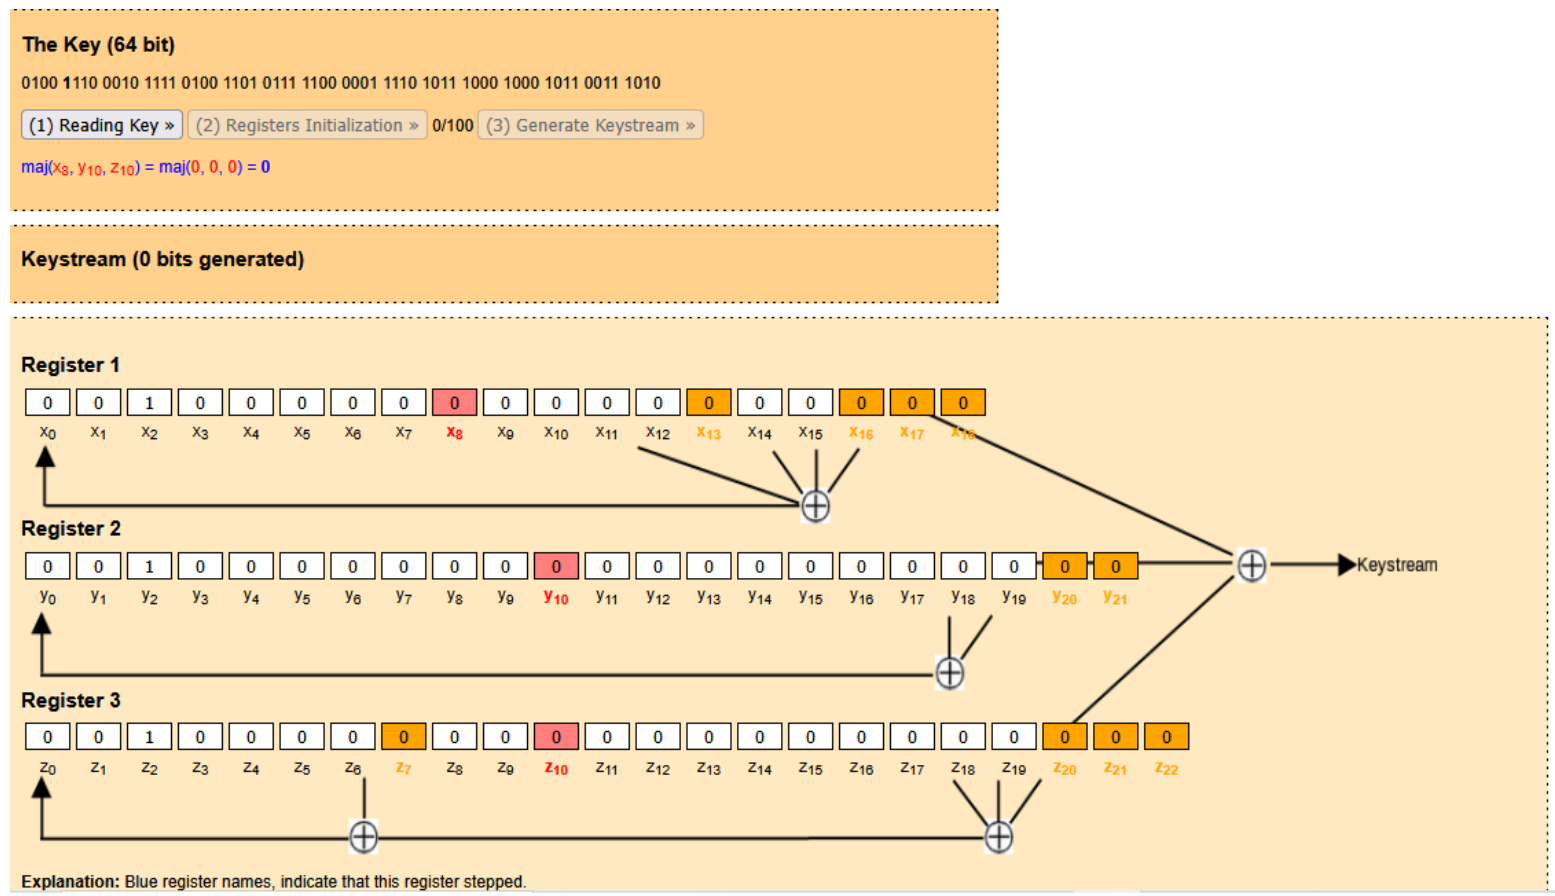
\includegraphics[width=170.10mm,height=246.51mm]{../../images/llm/page_073_img_01.png}%
\end{textblock*}

\end{document}
